\documentclass[12pt]{article}
\usepackage[a4paper,margin=1in]{geometry}
\usepackage{graphicx}
\usepackage{tikz}
\usepackage{lmodern}
\usepackage{xcolor}
\usepackage{fancyhdr}
\usepackage{helvet}
\renewcommand{\familydefault}{\sfdefault}

% Colors
\definecolor{bannerbg}{RGB}{0,0,0}
\definecolor{quotebg}{gray}{0.7}

% Header/Footer
\pagestyle{fancy}
\fancyhf{}
\fancyhead[R]{\textit{Computing for the Psychological Sciences}}
\fancyhead[L]{}
\fancyfoot[C]{}
\renewcommand{\headrulewidth}{0pt}
\renewcommand{\footrulewidth}{0pt}

\begin{document}
% Custom Title Page
\thispagestyle{empty}
\begin{tikzpicture}[remember picture,overlay]
    % Black banner
    \fill[bannerbg] (current page.north west) rectangle ([yshift=-4cm]current page.north east);
    % Logo (adjust path/size as needed)
    \node[anchor=north west, yshift=-0.5cm, xshift=1cm] at (current page.north west) {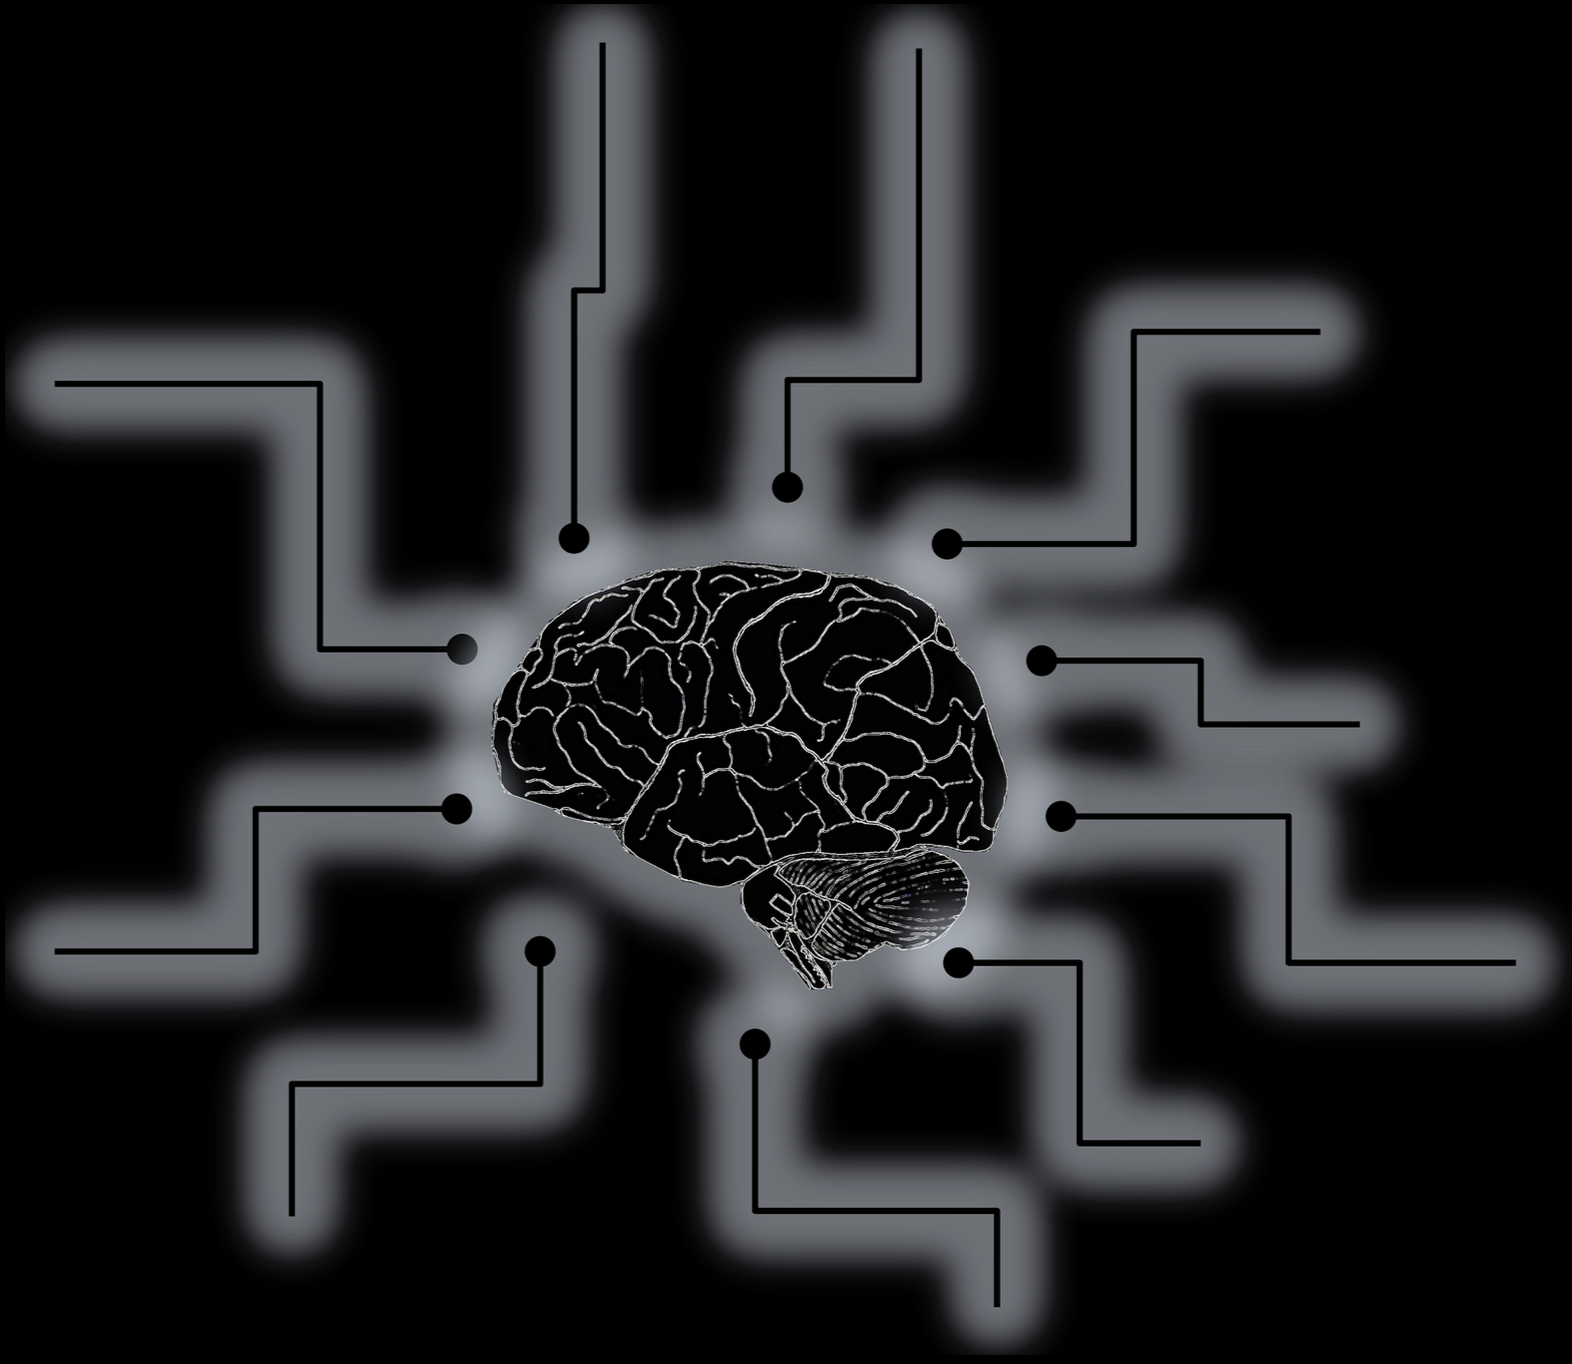
\includegraphics[height=3cm]{CAPSlogo.png}};
    % Title
    \node[anchor=north, text=white, font=\fontsize{36}{40}\selectfont, xshift=2cm] at ([yshift=-2cm]current page.north) {Introduction to LaTeX};
    % Page number (top right)
    \node[anchor=north east, font=\large, yshift=-0.5cm, xshift=-1cm] at (current page.north east) {1};
    % Quote background
    \fill[quotebg] ([yshift=-4cm]current page.north west) rectangle ([yshift=-5.2cm]current page.north east);
    % Quote text
    \node[anchor=north, align=center, font=\large, text=white] at ([yshift=-4.6cm]current page.north) {``Style means the right word. The rest matters little.''\\\textemdash~Jules Renard};
\end{tikzpicture}

% Add vertical space to push main content below the banner/quote
\vspace*{6.5cm}

% Main content
{\Huge \textbf{What is LaTeX?}}

\vspace{1em}

\noindent
\begin{minipage}{0.98\textwidth}
\large
LaTeX, pronounced ``Lay-tech'' or ``Lah-tech'', is a high-quality typesetting system; it includes features designed for the production of technical and scientific documentation. LaTeX is widely used in academia for the communication and publication of scientific documents in many fields, including mathematics, statistics, quantitative psychology, computer science, engineering, chemistry, physics, economics, linguistics, philosophy, and political science. It also has a prominent role in the preparation and publication of books and articles that contain complex elements. LaTeX is available for free at \texttt{https://www.latex-project.org/}.

\vspace{1em}
When using LaTeX, the writer uses plain text as opposed to the formatted text found in WYSIWYG (``what you see is what you get'') word processors like Microsoft Word, Google Docs, LibreOffice Writer and Apple Pages. In LaTeX, the writer uses markup tagging conventions to define the general structure of a document (such as article, book, and letter), to stylise text throughout a document (such as bold and italics), and to add citations and cross-references.
\end{minipage}

\end{document}
